\section{Developments in SpaghettiLens}

\subsection{Improved synthetic images}\label{subsec:sourcefit}

The mass maps produced by current implementation of SpaghettiLens are
based on images of point-like features.  No information about extended
images is used, except in so far as they help the user identify images
of point-like features.  The synthetic images offered to users are
rudimentary, corresponding to conical light profiles (that is,
circular light profiles with brightness decreasing linearly with radius).

We have now developed a prototype of better way to generate synthetic
images.  Figure~\figref{synthimg} illustrates.  First, areas
containing lensed images are selected (green frames in the figure).
The selected areas should be as free as possible from of light from
the lensing galaxy or from extraneous objects.  Pixels within the
selected areas are mapped to a grid on the source plane, using bending
angles given by the mass model.  The mapping from lens-plane pixels to
source-plane grid cells is many-to-one, because of image multiplicity
and magnification.  The brightness of each source-plane pixel is set
to the mean of all the lens-plane pixels mapping to it.  Finally, the
mapping is run back to the lens plane.  The result is a synthetic
image.  In effect, one is reconstructing a source-plane brightness map
by least-squares.

The procedure is not yet implemented in SpaghettiLens but can be
applied in post-processing.  The new synthetic images could be used to
improve the mass reconstruction, by weighting the ensemble of maps
according to how good the synthetic images are, but we have not
attempted to do so as yet.

\begin{figure}
  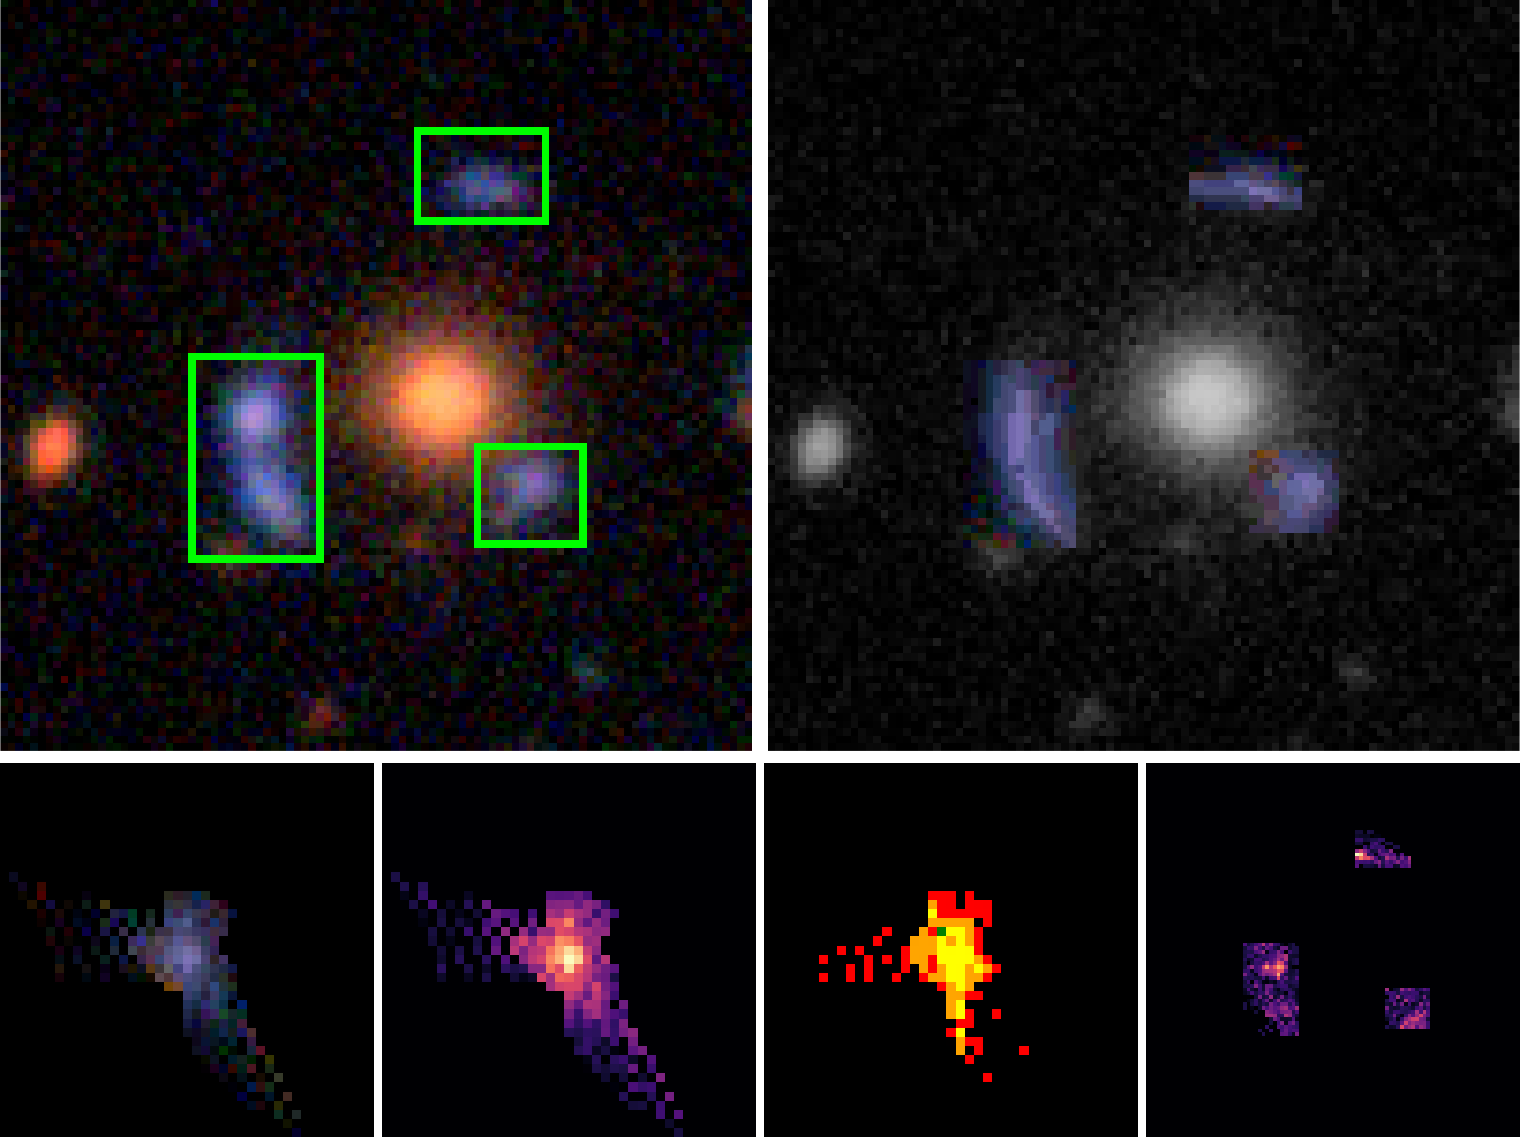
\includegraphics[width=\linewidth]{img/new_synth_img_detailed}
  \caption{Synthetic lensed image with source-profile fitting in SW05
    (J143454.4+522850). Top-left: original image, with areas
    containing lensed images enclosed within green frames.  Top-right:
    synthetic image (coloured arcs) with lensing galaxy and unrelated
    objects in greyscale.  Bottom from left to right: reconstructed
    source in colour, intensity (greyscale), count of lens plane
    pixels per source plane pixel, residual of original image to
    synthetic image.}
  \label{fig:synthimg}
\end{figure}

\subsection{Sub-sampling of central region}\label{subsec:hires}

The models of simulated lenses in \cite{2015MNRAS.447.2170K} showed a
tendency to be too shallow.  Allowing smaller mass tiles in the
central region, thus allowing the mass profile to rise more steeply
near the centre, was suggested as a possible cure.

Figure~\figref{subsampling} shows an experiment with smaller mass
tiles in the inner region.  Replacing the very central mass tile with
9 smaller tiles allows for steeper central profiles.  Doing the same
for the 25 innermost mass tiles allows for still steeper central
profiles, eliminating the systematic shallowness.  This is, however,
still not a completely satisfactory solution, because (a)~it increases
the number of mass tiles by 40\% and significantly increases the
computational time, and (b)~the square boundary between area with
different tile sizes is rather undesirable.
% 689 / 489 = 1.40899; in practice, runtime is more like x4 - x5!
% runtimes from logfiles: 87/22, 86/21, 85/16
The main modelling work in this paper was, however, done before the
experiments with smaller mass tiles was complete.  Some of the models
presented in this paper apply the intermediate option (corresponding
to the middle panel in Figure~\figref{subsampling}) while others use
the old system.  The results in this paper, however, mainly concern
the enclosed mass in the outer regions, so shallowness in the central
region should be inconsequential.

\begin{figure}
  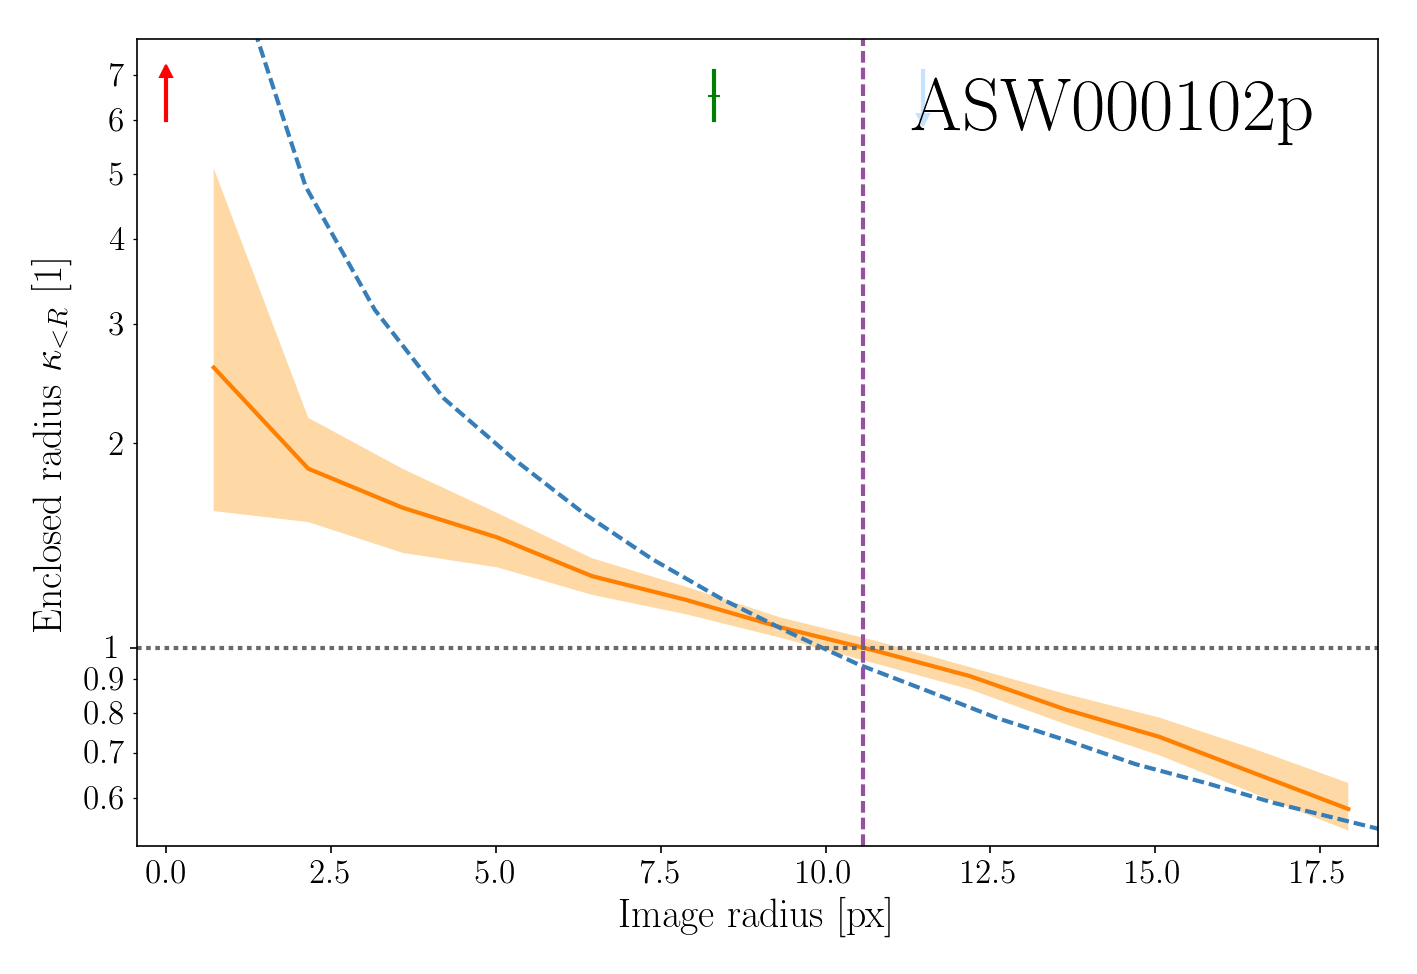
\includegraphics[width=.9\linewidth]{img/hires_comparison/ASW000102p_6941_11_hires_comparison}
  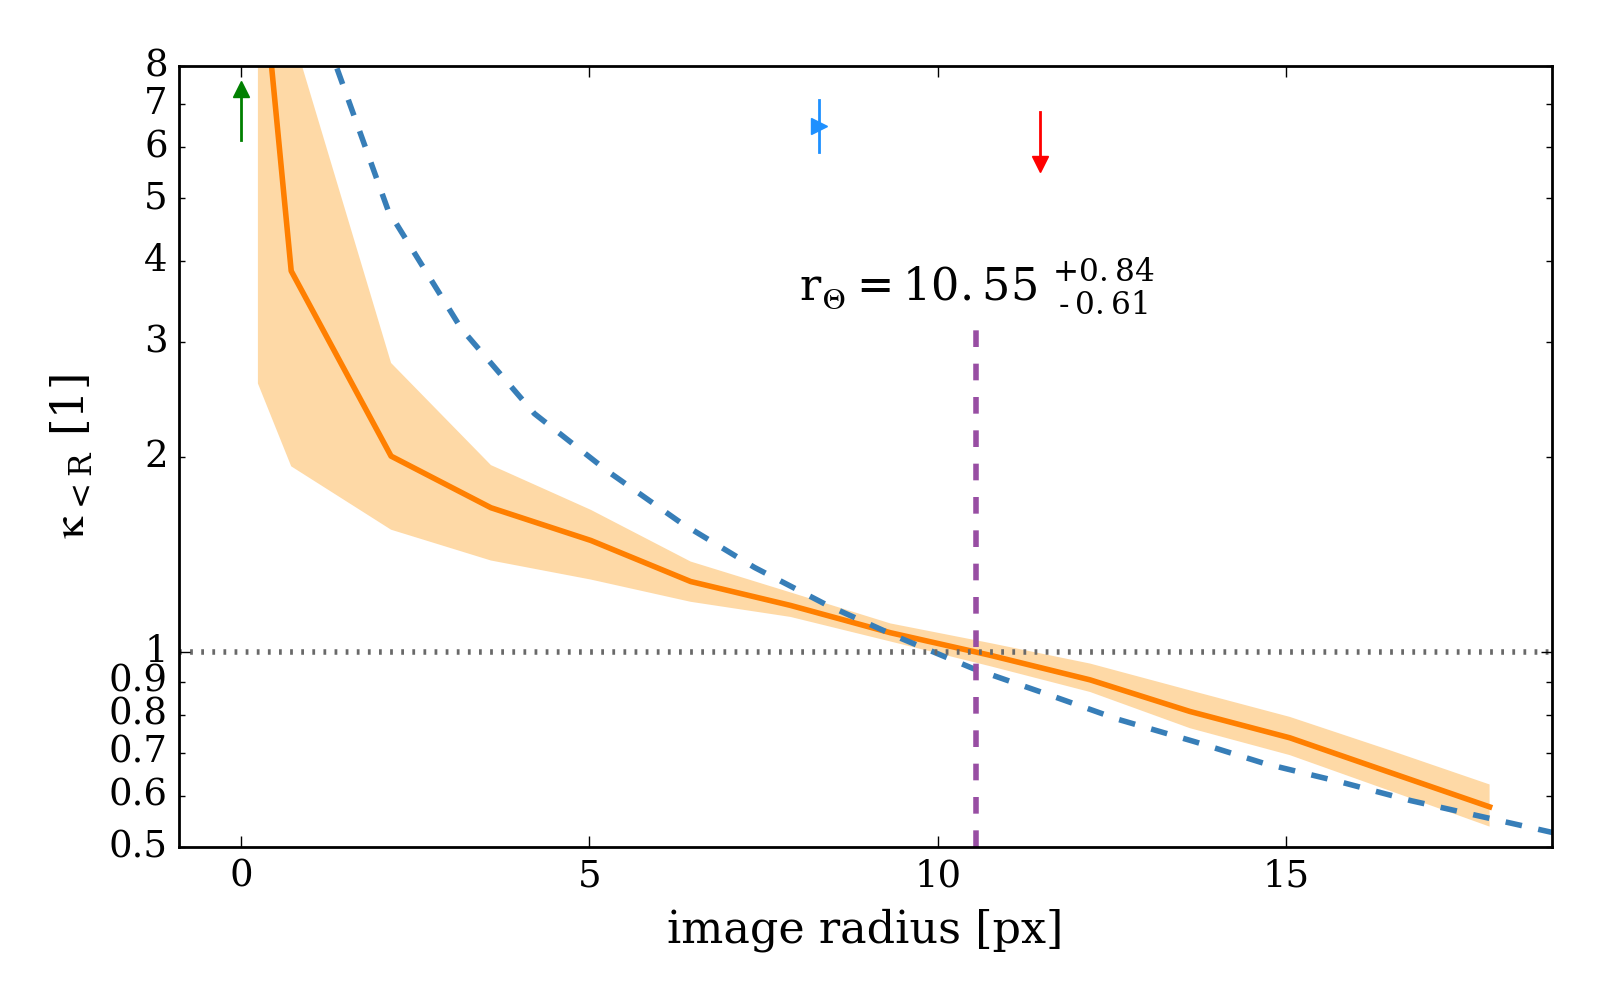
\includegraphics[width=.9\linewidth]{img/hires_comparison/ASW000102p_6941_13_hires_comparison}
  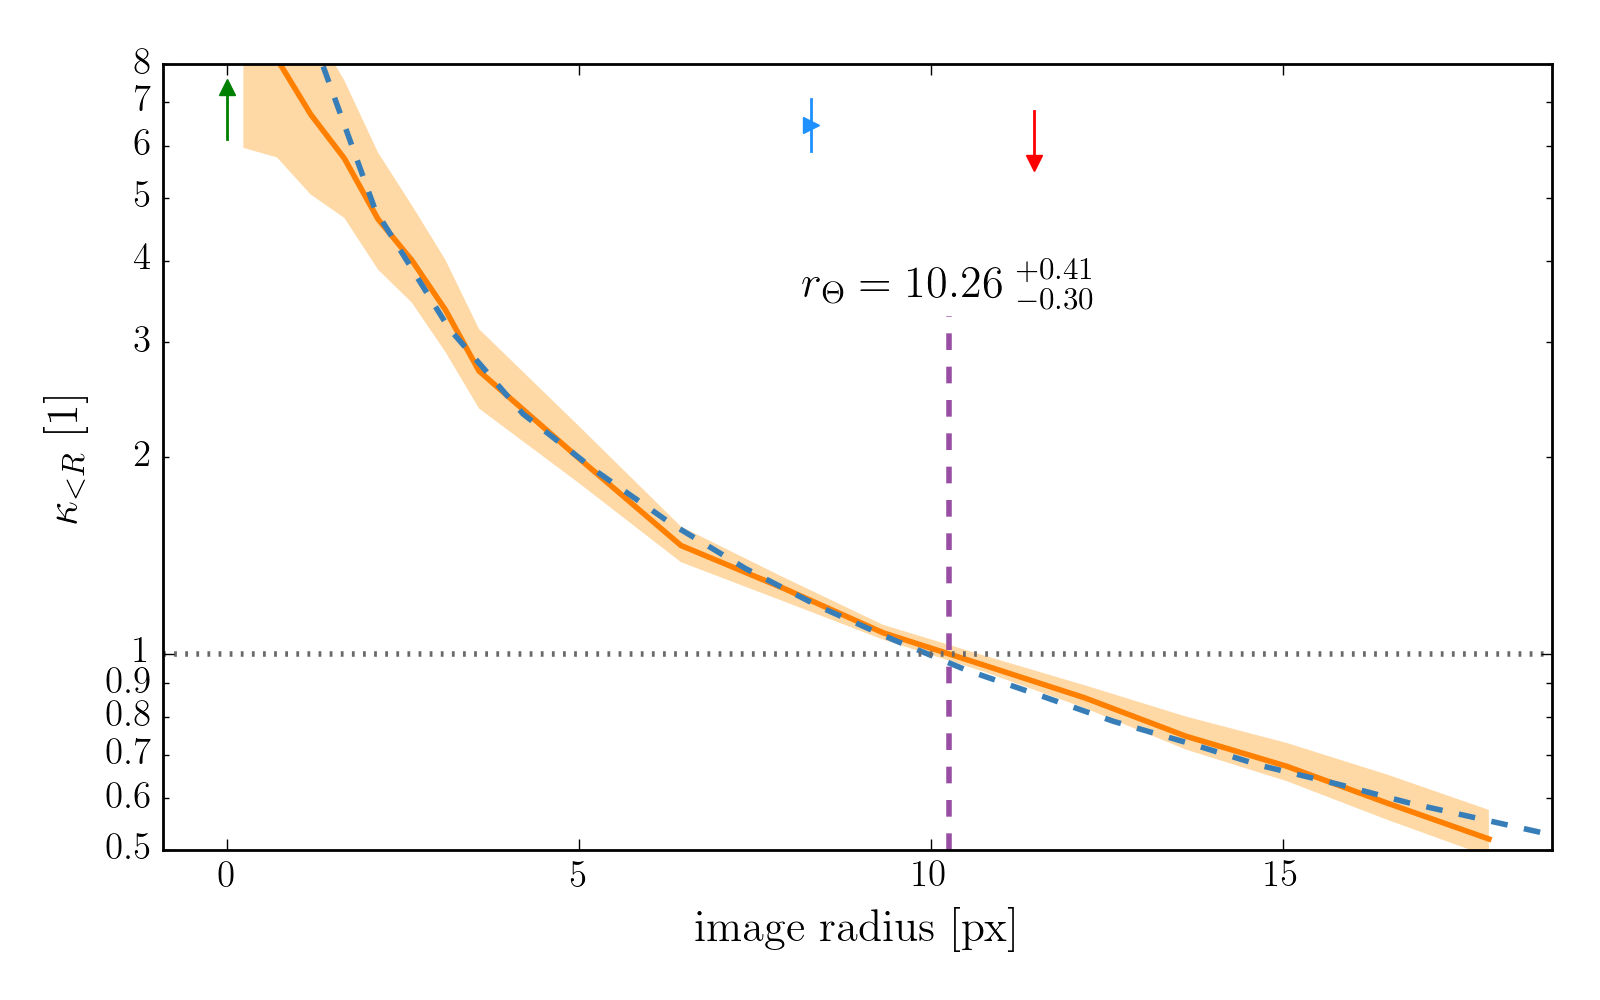
\includegraphics[width=.9\linewidth]{img/hires_comparison/ASW000102p_6941_33_hires_comparison}
  \caption{Model improvement resulting from using smaller mass tiles
    in the inner region of the mass model.  Shown here are the average
    enclosed $\kappa$ within a given projected radius, for three
    different reconstructions of a simulated lens (sim) from
    Space~Warps.  In each panel, the dashed blue curve is the correct
    answer.  The orange band represents the statistical ensemble from
    SpaghettiLens, the orange line being the ensemble mean.  Locations of
    images (maximum, saddle point, minimum) are marked with vertical
    arrows.  Crossing the horizontal $\kappa=1$ line is the effective
    Einstein radius \ER. The upper panel is from
    K\"ung et al., (2015) (see Figure~3 of that paper).  The middle
    panel is the result when the innermost mass tile is replaced by 9
    smaller tiles.  The lower panel results from replacing each of the
    innermost 5 by 5 tiles each with 9 smaller tiles.}
  \label{fig:subsampling}
\end{figure}

\subsection{Parameterisation of pixel models} \label{subsec:parameter}

In order to fit the set of pixelated models to a single parameterised model, a program was written that took a parameterised function and subtracted from it the mean and the principal components of the data, which were calculated using classical Principal Component Analysis.
This created the residuals function.
The number of components used in the analysis was varied, to test how this affected the output, and it was found that using 5 principle components tended to give a reasonable approximation.
A masking function was added which selected only the data points that fell inside the image of the lens, and the principal components were clipped in order to keep the values inside the region of the ensemble of models.
Any value higher than the clip was set to be the clip value.
This was chosen to be 2.5 as, assuming that the data follows a Gaussian error distribution, almost all the values for the variance should lie between 2 and 3 standard deviations from the mean.
Minimising the residuals function produces the set of parameters that fit the parameterised function to the original pixelated ensemble most closely.
A least squares fit was used to perform this minimisation.
The parameterised model function was obtained from the gravitational potential of an isothermal ellipsoid mass distribution \citep{2001astro.ph..2341K}.
This model is frequently used to describe gravitational lenses as it tends to fit well with observations.
The isothermal ellipsoid model outputs three useful parameters: the radius of the Einstein ring, the ellipticity of the model and the angle of the ellipticity from the vertical, giving the orientation of the galaxy.
By applying this model to simulated lenses for which the values of these parameters were already known, it was possible to gain an estimate of the projected accuracy of the results, before applying the model to the candidate lensing galaxies.

Preliminary results on recovery of Einstein radii are shown in
Figure~\ref{fig:parameter}.

\begin{figure}
  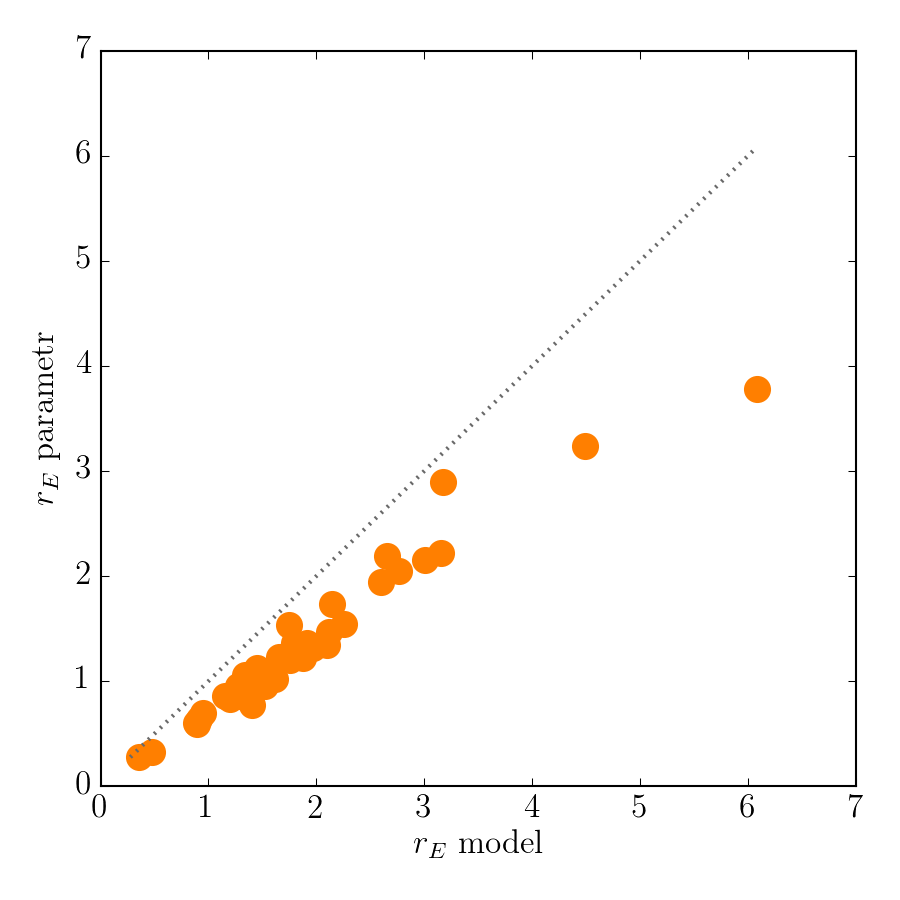
\includegraphics[width=\linewidth]{img/rE_comp/rE_comp.png}
  \caption{
    Comparison of Einstein radii \ER obtained from mass tiles directly to those obtained from a parameterized model to test the performance of the conversion algorythm.
    The parameterized model was generated using princible componant analysis on the ensemble of models.
    The blue dashed line represents a perfect recovery of \ER.
    }
  \label{fig:parameter}
\end{figure}



